\documentclass[varwidth, border=0pt]{standalone}

\usepackage{times}      % Loads the Times-Roman Fonts
\usepackage{mathptmx}   % Loads the Times-Roman Math Fonts
\usepackage{subcaption}
\usepackage[labelfont={bf,sf},%
labelsep=period,%
justification=centering,
labelformat=parens,labelsep=quad,skip=3pt,font=scriptsize]{caption}
\usepackage{graphicx}

\begin{document}
	
	\begin{figure}\centering
		\begin{subfigure}{0.5\linewidth}
			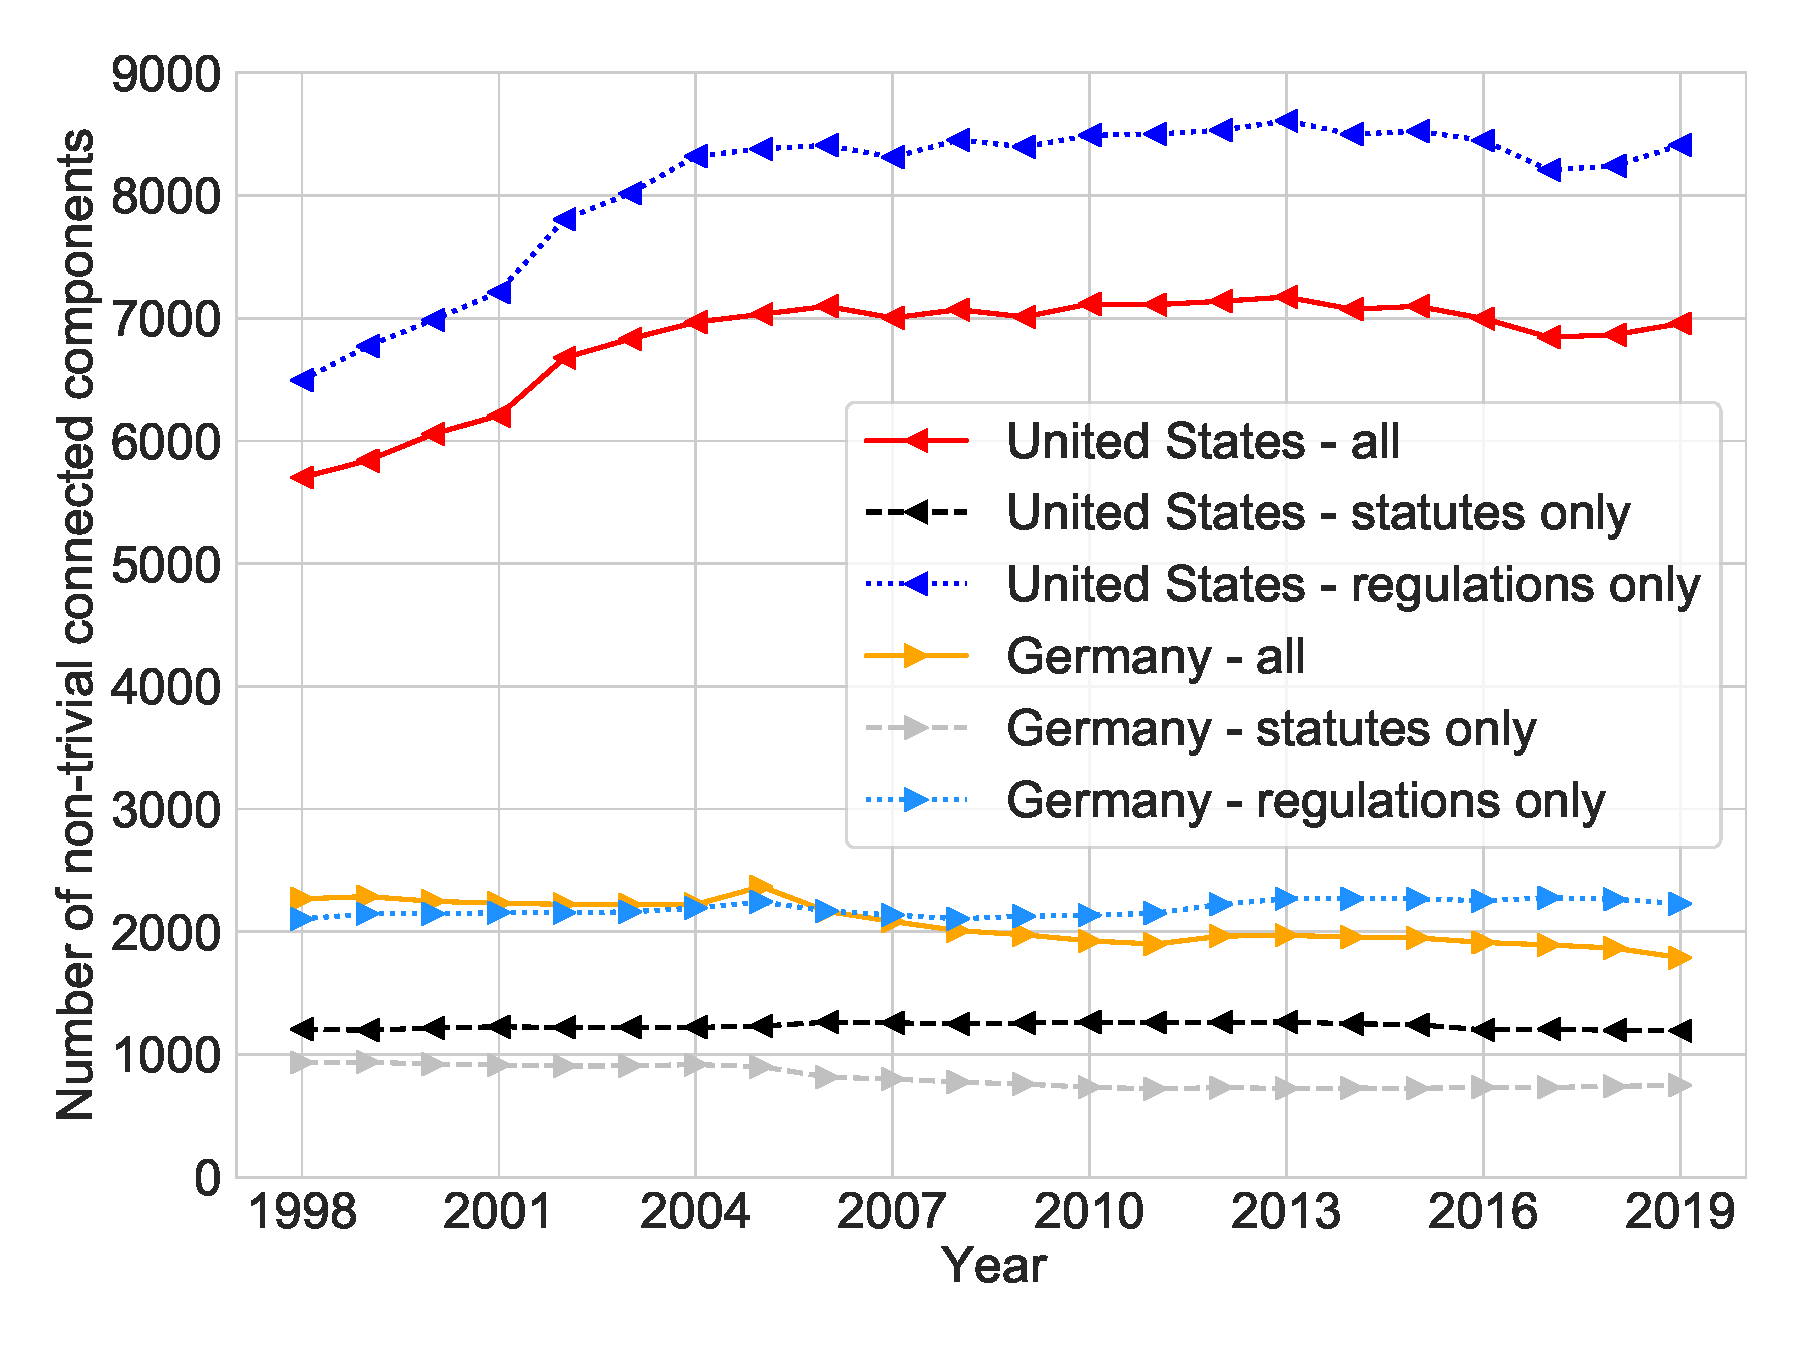
\includegraphics[width=\linewidth]{../../graphics/connectivity-number-of-components-comparison.pdf}
			\subcaption{Non-trivial connected components total}
		\end{subfigure}%
		\begin{subfigure}{0.5\linewidth}
			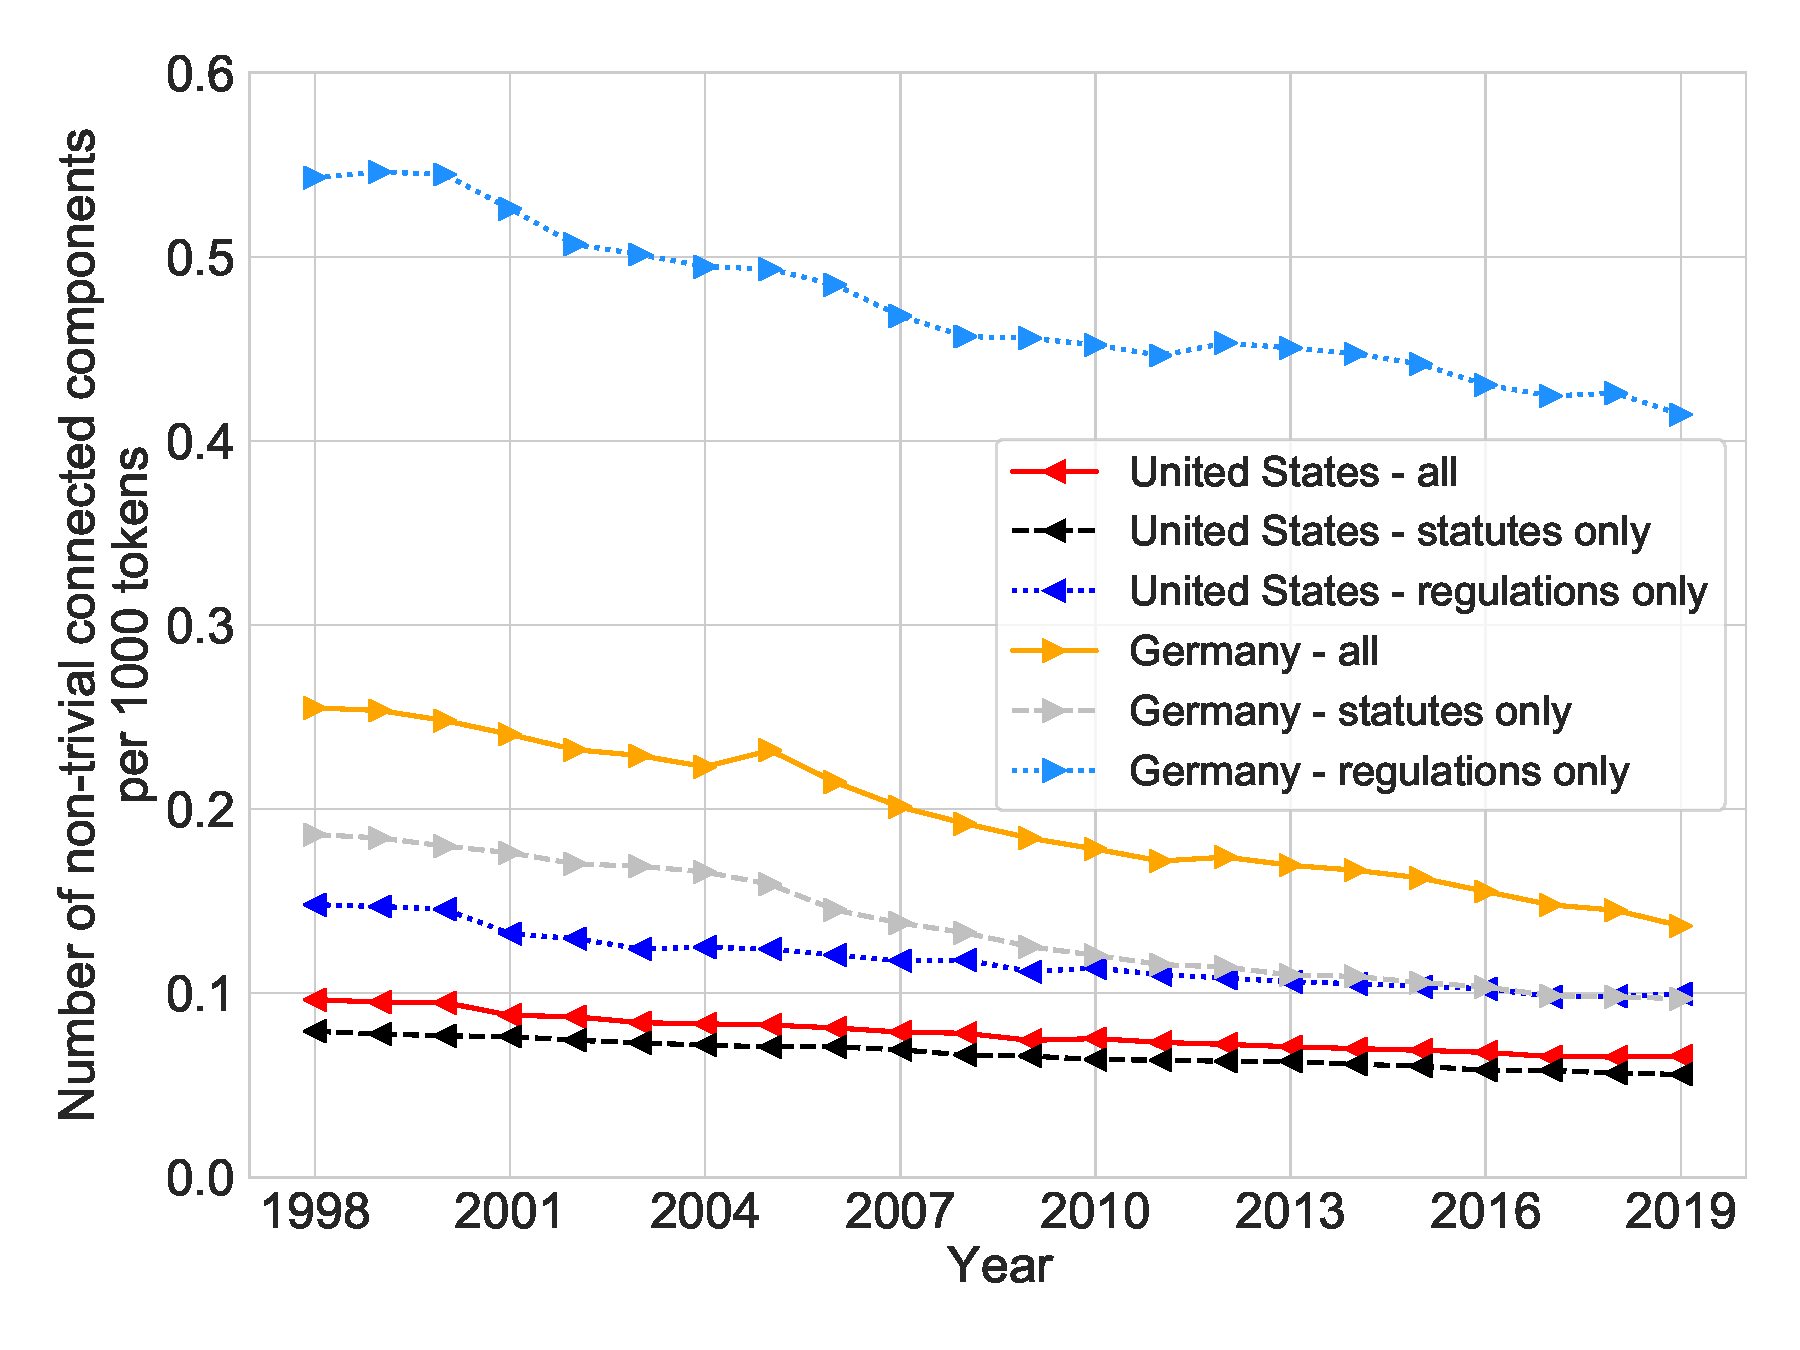
\includegraphics[width=\linewidth]{../../graphics/connectivity-number-of-components-comparison-rel.pdf}
			\subcaption{Non-trivial connected components per $1000$ tokens}
		\end{subfigure}
	\end{figure}
	
\end{document}